\documentclass[11pt,a3paper,landscape]{article}
\usepackage[utf8]{inputenc}
\usepackage[T1]{fontenc}
\usepackage[paperwidth=42cm,paperheight=29.7cm,margin=0.8cm]{geometry}
\usepackage{tikz}
\usepackage{graphicx}
\usetikzlibrary{arrows.meta,positioning,fit,backgrounds,calc}

\definecolor{districtFront}{RGB}{227,242,253}
\definecolor{districtBack}{RGB}{226,245,230}
\definecolor{districtLean}{RGB}{255,239,219}
\definecolor{districtInfra}{RGB}{236,230,252}
\definecolor{districtExternal}{RGB}{255,243,214}

\definecolor{roadRest}{RGB}{33,150,243}
\definecolor{roadSse}{RGB}{0,150,136}
\definecolor{roadCelery}{RGB}{239,108,0}
\definecolor{roadData}{RGB}{67,160,71}
\definecolor{roadGit}{RGB}{126,87,194}
\definecolor{roadInternal}{RGB}{90,90,90}

\begin{document}
\pagestyle{empty}

\begin{center}
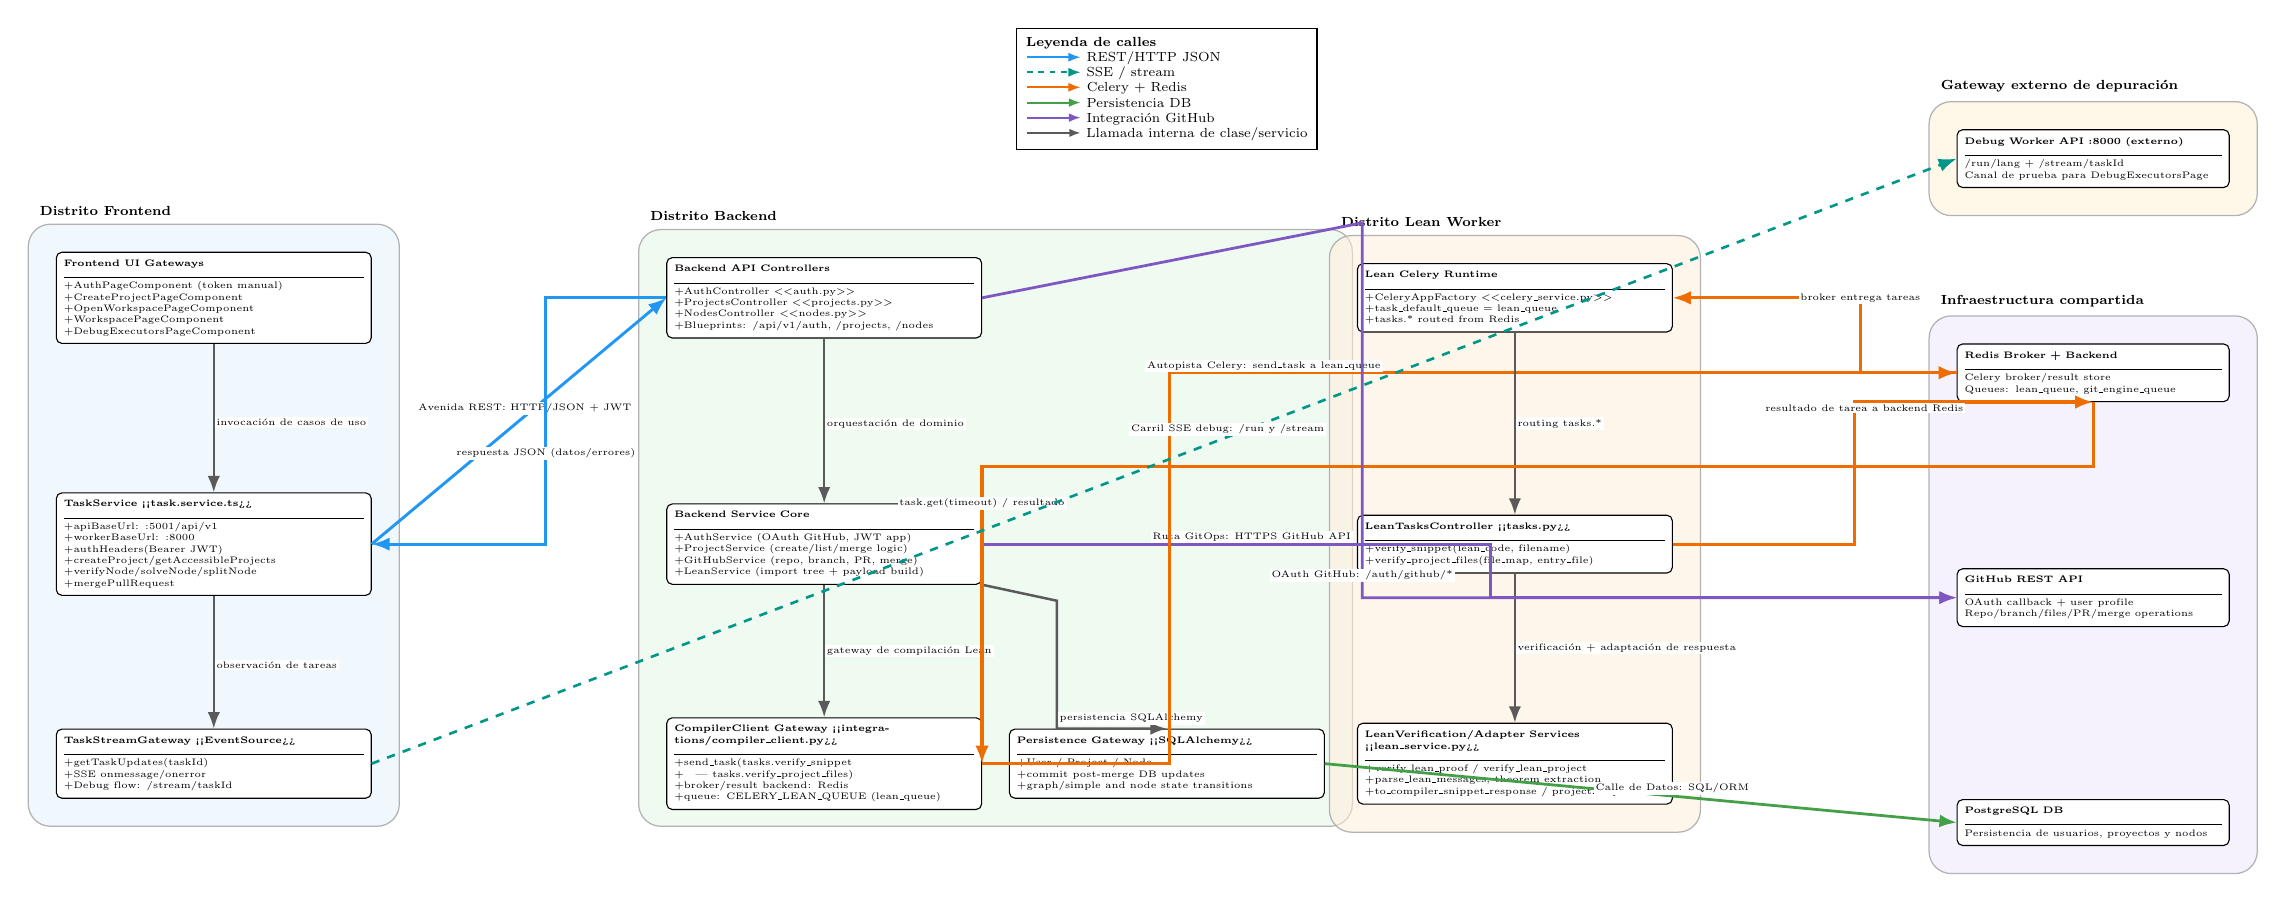
\begin{tikzpicture}[
  scale=0.68,
  transform shape,
  x=1cm,
  y=1cm,
  gateway/.style={
    draw,
    rounded corners=2pt,
    align=left,
    font=\tiny,
    text width=5.6cm,
    inner sep=4pt,
    fill=white
  },
  infra/.style={
    draw,
    rounded corners=2pt,
    align=left,
    font=\tiny,
    text width=4.8cm,
    inner sep=4pt,
    fill=white
  },
  district/.style={
    draw=black!30,
    line width=0.45pt,
    rounded corners=8pt,
    inner sep=10pt,
    fill opacity=0.55
  },
  rest/.style={-{Latex[length=2.3mm]}, line width=1.05pt, draw=roadRest},
  sse/.style={-{Latex[length=2.3mm]}, line width=0.95pt, draw=roadSse, dashed},
  celery/.style={-{Latex[length=2.3mm]}, line width=1.1pt, draw=roadCelery},
  data/.style={-{Latex[length=2.2mm]}, line width=1.0pt, draw=roadData},
  git/.style={-{Latex[length=2.2mm]}, line width=1.0pt, draw=roadGit},
  internal/.style={-{Latex[length=2.1mm]}, line width=0.9pt, draw=roadInternal},
  rel/.style={font=\tiny, fill=white, inner sep=1pt, text=black}
]

% =========================
% Frontend district
% =========================
\node[gateway] (uiFront) at (2.8,11.6) {
\textbf{Frontend UI Gateways}\\
\rule{\linewidth}{0.2pt}\\
+AuthPageComponent (token manual)\\
+CreateProjectPageComponent\\
+OpenWorkspacePageComponent\\
+WorkspacePageComponent\\
+DebugExecutorsPageComponent
};

\node[gateway] (taskService) at (2.8,7.0) {
\textbf{TaskService <<task.service.ts>>}\\
\rule{\linewidth}{0.2pt}\\
+apiBaseUrl: :5001/api/v1\\
+workerBaseUrl: :8000\\
+authHeaders(Bearer JWT)\\
+createProject/getAccessibleProjects\\
+verifyNode/solveNode/splitNode\\
+mergePullRequest
};

\node[gateway] (streamGateway) at (2.8,2.9) {
\textbf{TaskStreamGateway <<EventSource>>}\\
\rule{\linewidth}{0.2pt}\\
+getTaskUpdates(taskId)\\
+SSE onmessage/onerror\\
+Debug flow: /stream/{taskId}
};

% =========================
% Backend district
% =========================
\node[gateway] (apiBack) at (14.2,11.6) {
\textbf{Backend API Controllers}\\
\rule{\linewidth}{0.2pt}\\
+AuthController <<auth.py>>\\
+ProjectsController <<projects.py>>\\
+NodesController <<nodes.py>>\\
+Blueprints: /api/v1/auth, /projects, /nodes
};

\node[gateway] (serviceBack) at (14.2,7.0) {
\textbf{Backend Service Core}\\
\rule{\linewidth}{0.2pt}\\
+AuthService (OAuth GitHub, JWT app)\\
+ProjectService (create/list/merge logic)\\
+GitHubService (repo, branch, PR, merge)\\
+LeanService (import tree + payload build)
};

\node[gateway] (compilerGateway) at (14.2,2.9) {
\textbf{CompilerClient Gateway <<integrations/compiler\_client.py>>}\\
\rule{\linewidth}{0.2pt}\\
+send\_task(tasks.verify\_snippet\\
+\hspace*{6pt}| tasks.verify\_project\_files)\\
+broker/result backend: Redis\\
+queue: CELERY\_LEAN\_QUEUE (lean\_queue)
};

\node[gateway] (persistenceBack) at (20.6,2.9) {
\textbf{Persistence Gateway <<SQLAlchemy>>}\\
\rule{\linewidth}{0.2pt}\\
+User / Project / Node\\
+commit post-merge DB updates\\
+graph/simple and node state transitions
};

% =========================
% Lean district
% =========================
\node[gateway] (leanBoot) at (27.1,11.6) {
\textbf{Lean Celery Runtime}\\
\rule{\linewidth}{0.2pt}\\
+CeleryAppFactory <<celery\_service.py>>\\
+task\_default\_queue = lean\_queue\\
+tasks.* routed from Redis
};

\node[gateway] (leanTasks) at (27.1,7.0) {
\textbf{LeanTasksController <<tasks.py>>}\\
\rule{\linewidth}{0.2pt}\\
+verify\_snippet(lean\_code, filename)\\
+verify\_project\_files(file\_map, entry\_file)
};

\node[gateway] (leanService) at (27.1,2.9) {
\textbf{LeanVerification/Adapter Services <<lean\_service.py>>}\\
\rule{\linewidth}{0.2pt}\\
+verify\_lean\_proof / verify\_lean\_project\\
+parse\_lean\_messages, theorem extraction\\
+to\_compiler\_snippet\_response / project\_response
};

% =========================
% Infra / external district
% =========================
\node[infra] (redis) at (37.9,10.2) {
\textbf{Redis Broker + Backend}\\
\rule{\linewidth}{0.2pt}\\
Celery broker/result store\\
Queues: lean\_queue, git\_engine\_queue
};

\node[infra] (githubApi) at (37.9,6.0) {
\textbf{GitHub REST API}\\
\rule{\linewidth}{0.2pt}\\
OAuth callback + user profile\\
Repo/branch/files/PR/merge operations
};

\node[infra] (postgres) at (37.9,1.8) {
\textbf{PostgreSQL DB}\\
\rule{\linewidth}{0.2pt}\\
Persistencia de usuarios, proyectos y nodos
};

\node[infra] (debugWorker) at (37.9,14.2) {
\textbf{Debug Worker API :8000 (externo)}\\
\rule{\linewidth}{0.2pt}\\
/run/{lang} + /stream/{taskId}\\
Canal de prueba para DebugExecutorsPage
};

% =========================
% District background boxes
% =========================
\begin{scope}[on background layer]
  \node[district, fill=districtFront, fit=(uiFront)(streamGateway)] (bgFront) {};
  \node[district, fill=districtBack, fit=(apiBack)(persistenceBack)] (bgBack) {};
  \node[district, fill=districtLean, fit=(leanBoot)(leanService)] (bgLean) {};
  \node[district, fill=districtInfra, fit=(redis)(postgres)] (bgInfra) {};
  \node[district, fill=districtExternal, fit=(debugWorker)] (bgExternal) {};

  \node[font=\scriptsize\bfseries, anchor=south west] at ($(bgFront.north west)+(3pt,1pt)$) {Distrito Frontend};
  \node[font=\scriptsize\bfseries, anchor=south west] at ($(bgBack.north west)+(3pt,1pt)$) {Distrito Backend};
  \node[font=\scriptsize\bfseries, anchor=south west] at ($(bgLean.north west)+(3pt,1pt)$) {Distrito Lean Worker};
  \node[font=\scriptsize\bfseries, anchor=south west] at ($(bgInfra.north west)+(3pt,1pt)$) {Infraestructura compartida};
  \node[font=\scriptsize\bfseries, anchor=south west] at ($(bgExternal.north west)+(3pt,1pt)$) {Gateway externo de depuración};
\end{scope}

% =========================
% Street relations (communication vehicles)
% =========================
\draw[internal] (uiFront.south) -- (taskService.north)
  node[rel, pos=0.53, right] {invocación de casos de uso};

\draw[internal] (taskService.south) -- (streamGateway.north)
  node[rel, pos=0.52, right] {observación de tareas};

\draw[rest] (taskService.east) -- (apiBack.west)
  node[rel, pos=0.52, above] {Avenida REST: HTTP/JSON + JWT};

\draw[rest] (apiBack.west) -- ++(-2.25,0) |- (taskService.east)
  node[rel, pos=0.30, below] {respuesta JSON (datos/errores)};

\draw[internal] (apiBack.south) -- (serviceBack.north)
  node[rel, pos=0.52, right] {orquestación de dominio};

\draw[internal] (serviceBack.south) -- (compilerGateway.north)
  node[rel, pos=0.5, right] {gateway de compilación Lean};

\draw[internal] (serviceBack.south east) -- ++(1.4,-0.3) |- (persistenceBack.north)
  node[rel, pos=0.46, right] {persistencia SQLAlchemy};

\draw[git] (serviceBack.east) -- ++(9.5,0)
  node[rel, pos=0.53, above] {Ruta GitOps: HTTPS GitHub API} |- (githubApi.west);

\draw[data] (persistenceBack.east) -- (postgres.west)
  node[rel, pos=0.55, above] {Calle de Datos: SQL/ORM};

\draw[celery] (compilerGateway.east) -- ++(3.5,0) |- (redis.west)
  node[rel, pos=0.56, above] {Autopista Celery: send\_task a lean\_queue};

\draw[celery] (redis.west) -- ++(-1.8,0) |- (leanBoot.east)
  node[rel, pos=0.45, above] {broker entrega tareas};

\draw[internal] (leanBoot.south) -- (leanTasks.north)
  node[rel, pos=0.5, right] {routing tasks.*};

\draw[internal] (leanTasks.south) -- (leanService.north)
  node[rel, pos=0.5, right] {verificación + adaptación de respuesta};

\draw[celery] (leanTasks.east) -- ++(3.4,0) |- (redis.south)
  node[rel, pos=0.52, below] {resultado de tarea a backend Redis};

\draw[celery] (redis.south) -- ++(0,-1.2) -| (compilerGateway.east)
  node[rel, pos=0.55, below] {task.get(timeout) / resultado};

\draw[sse] (streamGateway.east) -- (debugWorker.west)
  node[rel, pos=0.54, above] {Carril SSE debug: /run y /stream};

\draw[git] (apiBack.east) -- ++(7.1,1.4) |- (githubApi.west)
  node[rel, pos=0.48, above] {OAuth GitHub: /auth/github/*};

% Legend
\node[draw, align=left, font=\scriptsize, inner sep=5pt, fill=white] at (20.6,15.5) (legend) {
\textbf{Leyenda de calles}\\
\tikz{\draw[rest] (0,0)--(1.0,0);} REST/HTTP JSON\\
\tikz{\draw[sse] (0,0)--(1.0,0);} SSE / stream\\
\tikz{\draw[celery] (0,0)--(1.0,0);} Celery + Redis\\
\tikz{\draw[data] (0,0)--(1.0,0);} Persistencia DB\\
\tikz{\draw[git] (0,0)--(1.0,0);} Integración GitHub\\
\tikz{\draw[internal] (0,0)--(1.0,0);} Llamada interna de clase/servicio
};

\end{tikzpicture}
\end{center}

\end{document}